\pagenumbering{arabic}
%\documentclass[slides]{beamer}
\documentclass[mathserif, 8pt]{beamer}
\usepackage[framesassubsections]{beamerprosper}
\setbeamercovered{transparent}
%\documentclass[slides,hyperref={pdfpagelabels=false}]{beamer}
%\documentclass[handout,gray]{beamer}
\usepackage[T1]{fontenc}
\usepackage[utf8]{inputenc}
\usepackage{textcomp}
\usepackage{verbatim}
\usepackage{amsbsy}
\usepackage{multirow}
\usepackage{multicol}
\usepackage{booktabs} % Make some nice tables
\usepackage{ae,aecompl}

%%%%%%%%%%%% COULEURS %%%%%%%%%%%%%%%%%%%%%%%%%%%

\mode<presentation>
{
  \definecolor{beamerstructure}{RGB}{43,79,112}
  \definecolor{sidebackground}{RGB}{230,242,250}
  \definecolor{CTCC}{RGB}{133,188,228}
  \color{beamerstructure}
  \usetheme{default}
  \usepackage{courier}
  \beamertemplateballitem
\setbeamertemplate{navigation symbols}{}
%\setbeamertemplate{sidebar left}{\thispdfpagelabel{\insertframenumber}}
%\setbeamertemplate{footline}{\quad\insertframenumber}
%\usecolortheme{CTCC}
}
\usebackgroundtemplate{\includegraphics[width=1.02\paperwidth]{../templets/ctcc_general.jpg}}

\title{\\\vspace{1cm}
A first attempt at multiresolution Orbital-Free DFT}
%\subtitle{\textcolor{magenta}{My subtitle (if applicable)}}
\author{Stig Rune Jensen}
\institute[CTCC]{\\[-6mm]stig.r.jensen@uit.no\\[6mm]UiT The Arctic University of Norway\\[6mm]
\includegraphics[height=1.5cm]{../templets/uio.pdf}\hspace{1cm} 
\includegraphics[height=1.5cm]{../templets/sff.pdf}\hspace{1cm}
\includegraphics[height=1.5cm]{../templets/uit.pdf}}
%\date{Troms\o, March 20th 2014}
\date{\today}

\newcommand{\gb}[1]{green!#1!black}
\newcommand{\rb}[1]{red!#1!black}
\newcommand{\bb}[1]{blue!#1!black}
\newcommand{\coleq}{red!60!black}
\newcommand{\du}{\textrm{d}}

\newcommand{\mydef}{\stackrel{\text{def}}{\hbox{=}}} 

\begin{document}

\footnotesize
\setlength{\unitlength}{\textwidth}

{
\usebackgroundtemplate{\includegraphics[width=1.02\paperwidth]{../templets/ctcc_forside.jpg}}
\maketitle
}

%\begin{frame}
    %\frametitle{The molecular Schr\"{o}dinger equation}
    %\ \\
    %\begin{equation}
	%\nonumber
	%\hat{H}\psi = E\psi
    %\end{equation}
    %\ \\
    %\begin{equation}
	%\nonumber
	%\hat{H} =   -\sum_I \frac{\nabla^2}{2M_I} - \sum_i \frac{\nabla^2}{2}
		    %+\sum_{I>J} \frac{Z_IZ_J}{|\boldsymbol{R}_I-\boldsymbol{R}_J|} 
		    %-\sum_{i,I} \frac{Z_I}{|\boldsymbol{r}_i-\boldsymbol{R}_I|} 
		    %+\sum_{i>j} \frac{1}{|\boldsymbol{r}_i-\boldsymbol{r}_j|} 
    %\end{equation}
    %\ \\
    %\ \\
    %\ \\
    %\centering
    %For an $N$-particle problem, the wave function is $3N$-dimensional
    %\begin{equation}
	%\nonumber
	%\psi = \psi(\boldsymbol{r}_1,\boldsymbol{r}_2,\dots,\boldsymbol{r}_N)
    %\end{equation}
    %\ \\
    %\ \\
    %\ \\
    %\centering
    %$\beta$-Carotene ($C_{40}H_{56}$) has 296 electrons and an 888-dimensional wave function!
    %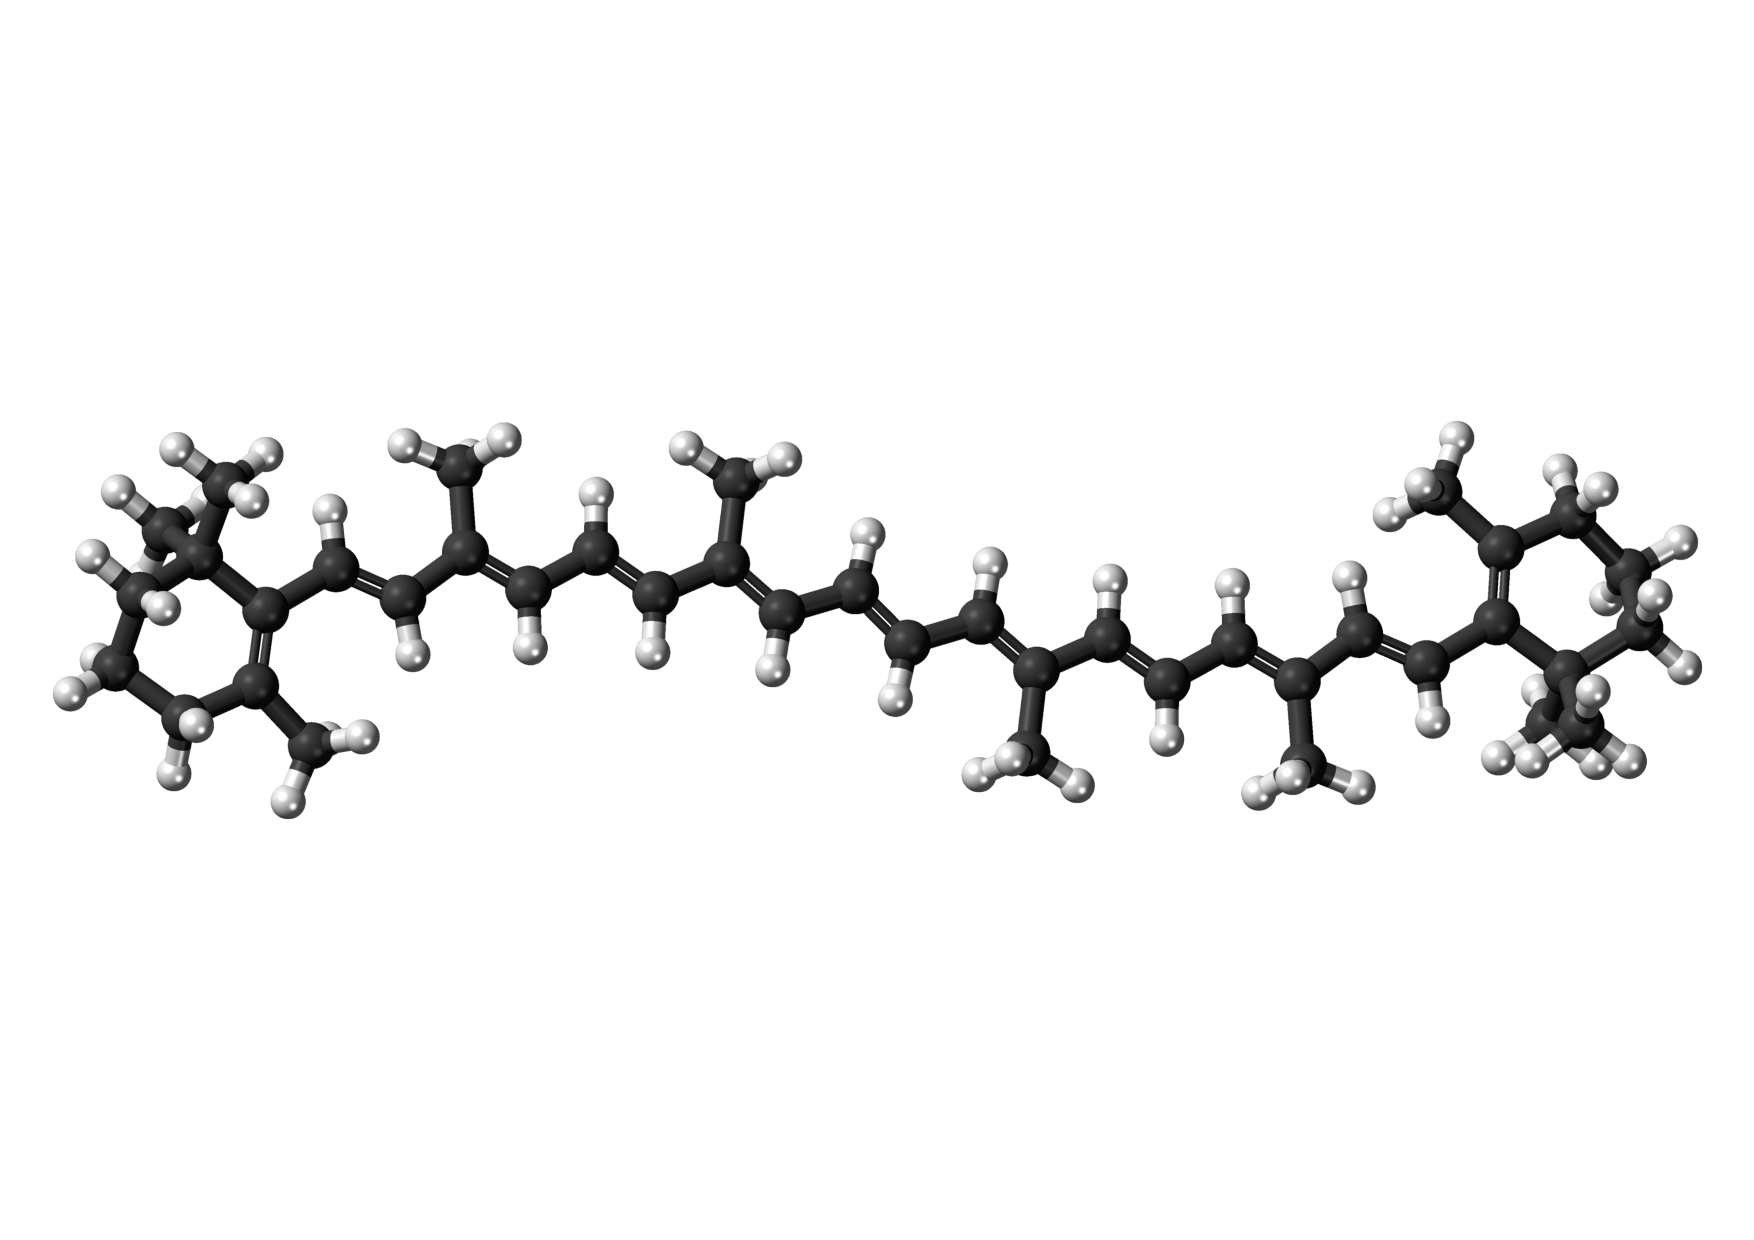
\includegraphics[scale=0.3, clip, viewport = 0 150 900 430]{figures/beta-carotene.pdf}
%\end{frame}

\begin{frame}
    \frametitle{Density Functional Theory}
    \centering
    \textbf{Dramatically reduce the dimensionality of the problem}
    \begin{equation}
	\nonumber
	\rho(\boldsymbol{r}_1) = N \int |\psi(\boldsymbol{r}_1, \boldsymbol{r}_2,\dots,
	\boldsymbol{r}_N)|^2 d\boldsymbol{r}_2\cdots d\boldsymbol{r}_N
    \end{equation}
    \ \\
    \ \\
    \ \\
    \textbf{Energy expressed as functional of the density}
    \begin{equation}
	\nonumber
	E[\rho] = T[\rho] + V_{ne}[\rho] + V_{ee}[\rho]
    \end{equation}
    \ \\
    \ \\
    \ \\
    \begin{itemize}
	\item	Electron-nuclear energy \textbf{is known} (within Born-Oppenheimer) as the classical Coulomb interaction
	\item	Quantum mechanical electron-electron energy \textbf{is not known} (classical Coulomb, exchange and correlation)
	\item	Kinetic energy of interacting electrons \textbf{is not known}
    \end{itemize}
    \ \\
    \ \\
    \ \\
    \begin{columns}
    \begin{column}{.50\textwidth}
    \centering
    \textbf{Classical Coulomb energies}
    \begin{align}
	\nonumber
	&\\
	\nonumber
	V_{ne}[\rho] &= \int \rho(\boldsymbol{r})v_{nuc}(\boldsymbol{r})d\boldsymbol{r}\\
	\nonumber
	&\\
	\nonumber
	V_{ee}[\rho] \approx J[\rho] &= \frac{1}{2} \int \rho(\boldsymbol{r})v_{el}(\boldsymbol{r})d\boldsymbol{r}
    \end{align}
    \end{column}
    \begin{column}{.50\textwidth}
    \centering
    \textbf{Classical Coulomb potentials}
    \begin{align}
	\nonumber
	&\\
	\nonumber
	v_{nuc}(\boldsymbol{r}) &= -\sum_I\frac{Z_I}{|\boldsymbol{r}-\boldsymbol{R}_I|}\\
	\nonumber
	&\\
	\nonumber
	v_{el}(\boldsymbol{r}) &= \int \frac{\rho(\boldsymbol{r}')}{4\pi|\boldsymbol{r}-\boldsymbol{r}'|} d\boldsymbol{r}'
    \end{align}
    \end{column}
    \end{columns}    
\end{frame}

\begin{frame}
    \frametitle{Kohn-Sham DFT}
    \begin{columns}
    \begin{column}{.50\textwidth}
    \centering
    \textbf{Express density through one-electron orbitals}
    \begin{equation}
	\nonumber
	\rho(\boldsymbol{r}) = \sum_i |\phi_i(\boldsymbol{r})|^2
    \end{equation}
    \end{column}
    \begin{column}{.50\textwidth}
    \centering
    \textbf{Known non-interacting kinetic energy}
    \begin{equation}
	\nonumber
	T_s[\lbrace\phi_i\rbrace] = \sum_i \left<\phi_i\left|-\frac{1}{2}\nabla^2\right|\phi_i\right>
    \end{equation}
    \end{column}
    \end{columns}
    \ \\
    \ \\
    \centering
    \textbf{Re-arrange the energy expression}
    \begin{equation}
	\nonumber
	E[\rho] = T_s[\lbrace\phi_i\rbrace] + V_{ne}[\rho] + J[\rho] + E_{xc}[\rho]
    \end{equation}
    \ \\
    \ \\
    \ \\
    \begin{itemize}
	\item	All unknown contributions are included in the (relatively small) exchange-correlation term
	\item	Minimization of the energy leads to one three-dimensional Euler equation
	\item	Equivalent to solving the coupled Kohn-Sham equations for non-interacting electrons
    \end{itemize}
    \ \\
    \ \\
    \ \\
    \begin{columns}
    \begin{column}{.50\textwidth}
    \centering
    \textbf{KS-DFT Euler equation}
    \begin{align}
	\nonumber
	\mu &=
	\frac{\delta T_s[\lbrace\phi_i\rbrace]}{\delta \rho(\boldsymbol{r})} + 
	\frac{\delta V_{en}[\rho]}{\delta \rho(\boldsymbol{r})} + 
	\frac{\delta J[\rho]}{\delta \rho(\boldsymbol{r})} + 
	\frac{\delta E_{xc}[\rho]}{\delta \rho(\boldsymbol{r})}\\
	\nonumber
	&= \frac{\delta T_s[\lbrace\phi_i\rbrace]}{\delta \rho(\boldsymbol{r})} + v_{KS}(\boldsymbol{r})
    \end{align}
    \end{column}
    \begin{column}{.50\textwidth}
    \centering
    \textbf{Effective Kohn-Sham potential}
    \begin{align}
	\nonumber
	v_{KS}(\boldsymbol{r}) &= 
	v_{nuc}(\boldsymbol{r}) + v_{el}(\boldsymbol{r}) + v_{xc}(\boldsymbol{r})\\
	\nonumber
				&\\
	\nonumber
				&=
	\frac{\delta V_{en}[\rho]}{\delta \rho(\boldsymbol{r})} + 
	\frac{\delta J[\rho]}{\delta \rho(\boldsymbol{r})} + 
	\frac{\delta E_{xc}[\rho]}{\delta \rho(\boldsymbol{r})}
    \end{align}
    \end{column}
    \end{columns}
    \ \\
    \ \\
    \ \\
    \centering
    \textbf{Kohn-Sham equations}
    \begin{equation}
	\nonumber
	\left[-\frac{1}{2}\nabla^2 + v_{KS}(\boldsymbol{r})\right]\phi_i(\boldsymbol{r}) = 
	\epsilon_i\phi_i(\boldsymbol{r})
    \end{equation}
\end{frame}

\begin{frame}
    \frametitle{Orbital-Free DFT}
    \centering
    \textbf{Keep the notion of non-interacting electrons}
    \begin{equation}
	\nonumber
	E[\rho] = T_s[\rho] + V_{ne}[\rho] + J[\rho] + E_{xc}[\rho]
    \end{equation}
    \ \\
    \ \\
    \begin{columns}
    \begin{column}{.40\textwidth}
	\centering
	\textbf{One-point functionals}
	\begin{equation}
	    \nonumber
	    T_s[\rho] = \int t_s(\rho;\boldsymbol{r}) d\boldsymbol{r}
	\end{equation}
    \end{column}
    \begin{column}{.60\textwidth}
	\centering
	\textbf{Two-point functionals}
	\begin{equation}
	    \nonumber
	    T_s[\rho] = \int \int f_1(\rho;\boldsymbol{r})\chi(\boldsymbol{r},\boldsymbol{r}') f_2(\rho;\boldsymbol{r}') d\boldsymbol{r}d\boldsymbol{r}'
	\end{equation}
    \end{column}
    \end{columns}
    \ \\
    \ \\
    \ \\
    \begin{itemize}
	\item	Able to treat very large systems ($10^4-10^6$ atoms) with good accuracy for metallic systems
	\item	In general not accurate enough for treatment of atomic and molecular systems
	\item	Gradient-corrected functionals \textbf{required} to achieve molecular binding
	\item	Two-point functionals are more complicated but are able to reproduce shell structure of atoms
    \end{itemize}
    \ \\
    \ \\
    \ \\
    \begin{columns}
    \begin{column}{.50\textwidth}
	\centering
	\textbf{Thomas-Fermi kinetic functional}
	\begin{equation}
	    \nonumber
	    T_{TF}[\rho] = \frac{3}{10}\left(3\pi^2\right)^{2/3}\int \rho^{5/3}(\boldsymbol{r}) d\boldsymbol{r}
	\end{equation}
    \end{column}
    \begin{column}{.50\textwidth}
	\centering
	\textbf{von Weizs\"{a}cker kinetic functional}
	\begin{equation}
	    \nonumber
	    T_{W}[\rho] = \frac{1}{8}\int \frac{|\nabla\rho(\boldsymbol{r})|^2}{\rho(\boldsymbol{r})} d\boldsymbol{r}
	\end{equation}
    \end{column}
    \end{columns}
    \ \\
    \ \\
    \ \\
    \centering
    \textbf{Borgoo-Tozer kinetic functional}
    \begin{equation}
        \nonumber
        T_{BT}[\rho] = \beta \int \rho^{5/3}(\boldsymbol{r})\left(\frac{|\nabla\rho(\boldsymbol{r})|}{\rho^{4/3}(\boldsymbol{r})}\right)^q d\boldsymbol{r}
    \end{equation}
\end{frame}

\begin{frame}
    \frametitle{The Euler equation}
    \centering
    \textbf{Separate kinetic energy into von Weizs\"{a}cker plus Pauli}
    \begin{equation}
	\nonumber
	T_s[\rho] = T_W[\rho] + T_\theta[\rho],\qquad \qquad T_\theta[\rho] \geq 0
    \end{equation}
    \ \\
    \ \\
    \ \\
    \begin{columns}
    \begin{column}{.50\textwidth}
	\centering
	\textbf{OF-DFT Euler equation}
	\begin{equation}
	    \nonumber
	    \mu = \frac{\delta T_W[\rho]}{\delta \rho(\boldsymbol{r})} +
	    \frac{\delta T_\theta[\rho]}{\delta\rho(\boldsymbol{r})} + v_{KS}(\boldsymbol{r})
	\end{equation}
    \end{column}
    \begin{column}{.50\textwidth}
	\centering
	\textbf{von Weizs\"{a}cker derivative}
	\begin{equation}
	    \nonumber
	    \frac{\delta T_{W}[\rho]}{\delta\rho(\boldsymbol{r})} = \frac{1}{\sqrt{\rho(\boldsymbol{r})}} 
	    \left(-\frac{1}{2}\nabla^2\right)\sqrt{\rho(\boldsymbol{r})}
	\end{equation}
    \end{column}
    \end{columns}
    \ \\
    \ \\
    \ \\
    \begin{itemize}
	\item	The von Weizs\"{a}cker term brings the Euler equation into Kohn-Sham form with one ''orbital''
	\item	''$\dots$\textbf{can be solved} iteratively to self-consistency \textbf{by any} Kohn-Sham computer program''$^\dag$ 
	\item	''The iterative self-consistent procedure used in Kohn-Sham calculations \textbf{does not work}, $\dots$''$^\ddag$
	\item	The purely repulsive Pauli term makes convergence non-trivial
    \end{itemize}
    \ \\
    \ \\
    \ \\
    \centering
    \textbf{One-orbital Kohn-Sham equation}
    \begin{equation}
        \nonumber
	\left[-\frac{1}{2}\nabla^2 + v_\theta(\boldsymbol{r}) + v_{KS}(\boldsymbol{r})\right]\sqrt{\rho(\boldsymbol{r})} = 
	\mu\sqrt{\rho(\boldsymbol{r})}
    \end{equation}
    \ \\
    \ \\
    \ \\
    \ \\
    \ \\
    \ \\
    $^\dag$\tiny{Levy, Perdew, Sahni, \it{Phys. Rev. A} \textbf{30}, 2745 (1984)}\\
    $^\ddag$\tiny{Chan, Cohen, Handy, \it{J. Chem. Phys.} \textbf{114}, 631 (2001)}
\end{frame}

\begin{frame}
    \frametitle{MRChem}
    \begin{columns}
    \begin{column}{.5\textwidth}
	\ \ \ \ \textbf{Multiwavelets}
	\begin{itemize}
	    \item   Real-space divided into cubic cells
	    \item   Low-order polynomial basis
	    \item   Adaptive multiresolution grids
	\end{itemize}
    \end{column}
    \begin{column}{.5\textwidth}
	\ \ \ \ \textbf{Features}
	\begin{itemize}
	    \item   Guaranteed accuracy (basis set limit)
	    \item   Linear scaling application of integral operators
	    \item   Efficiently parallelized using hybrid MPI/OpenMP
	\end{itemize}
    \end{column}
    \end{columns}
    \ \\
    \ \\
    \ \\
    \ \\
    \centering
    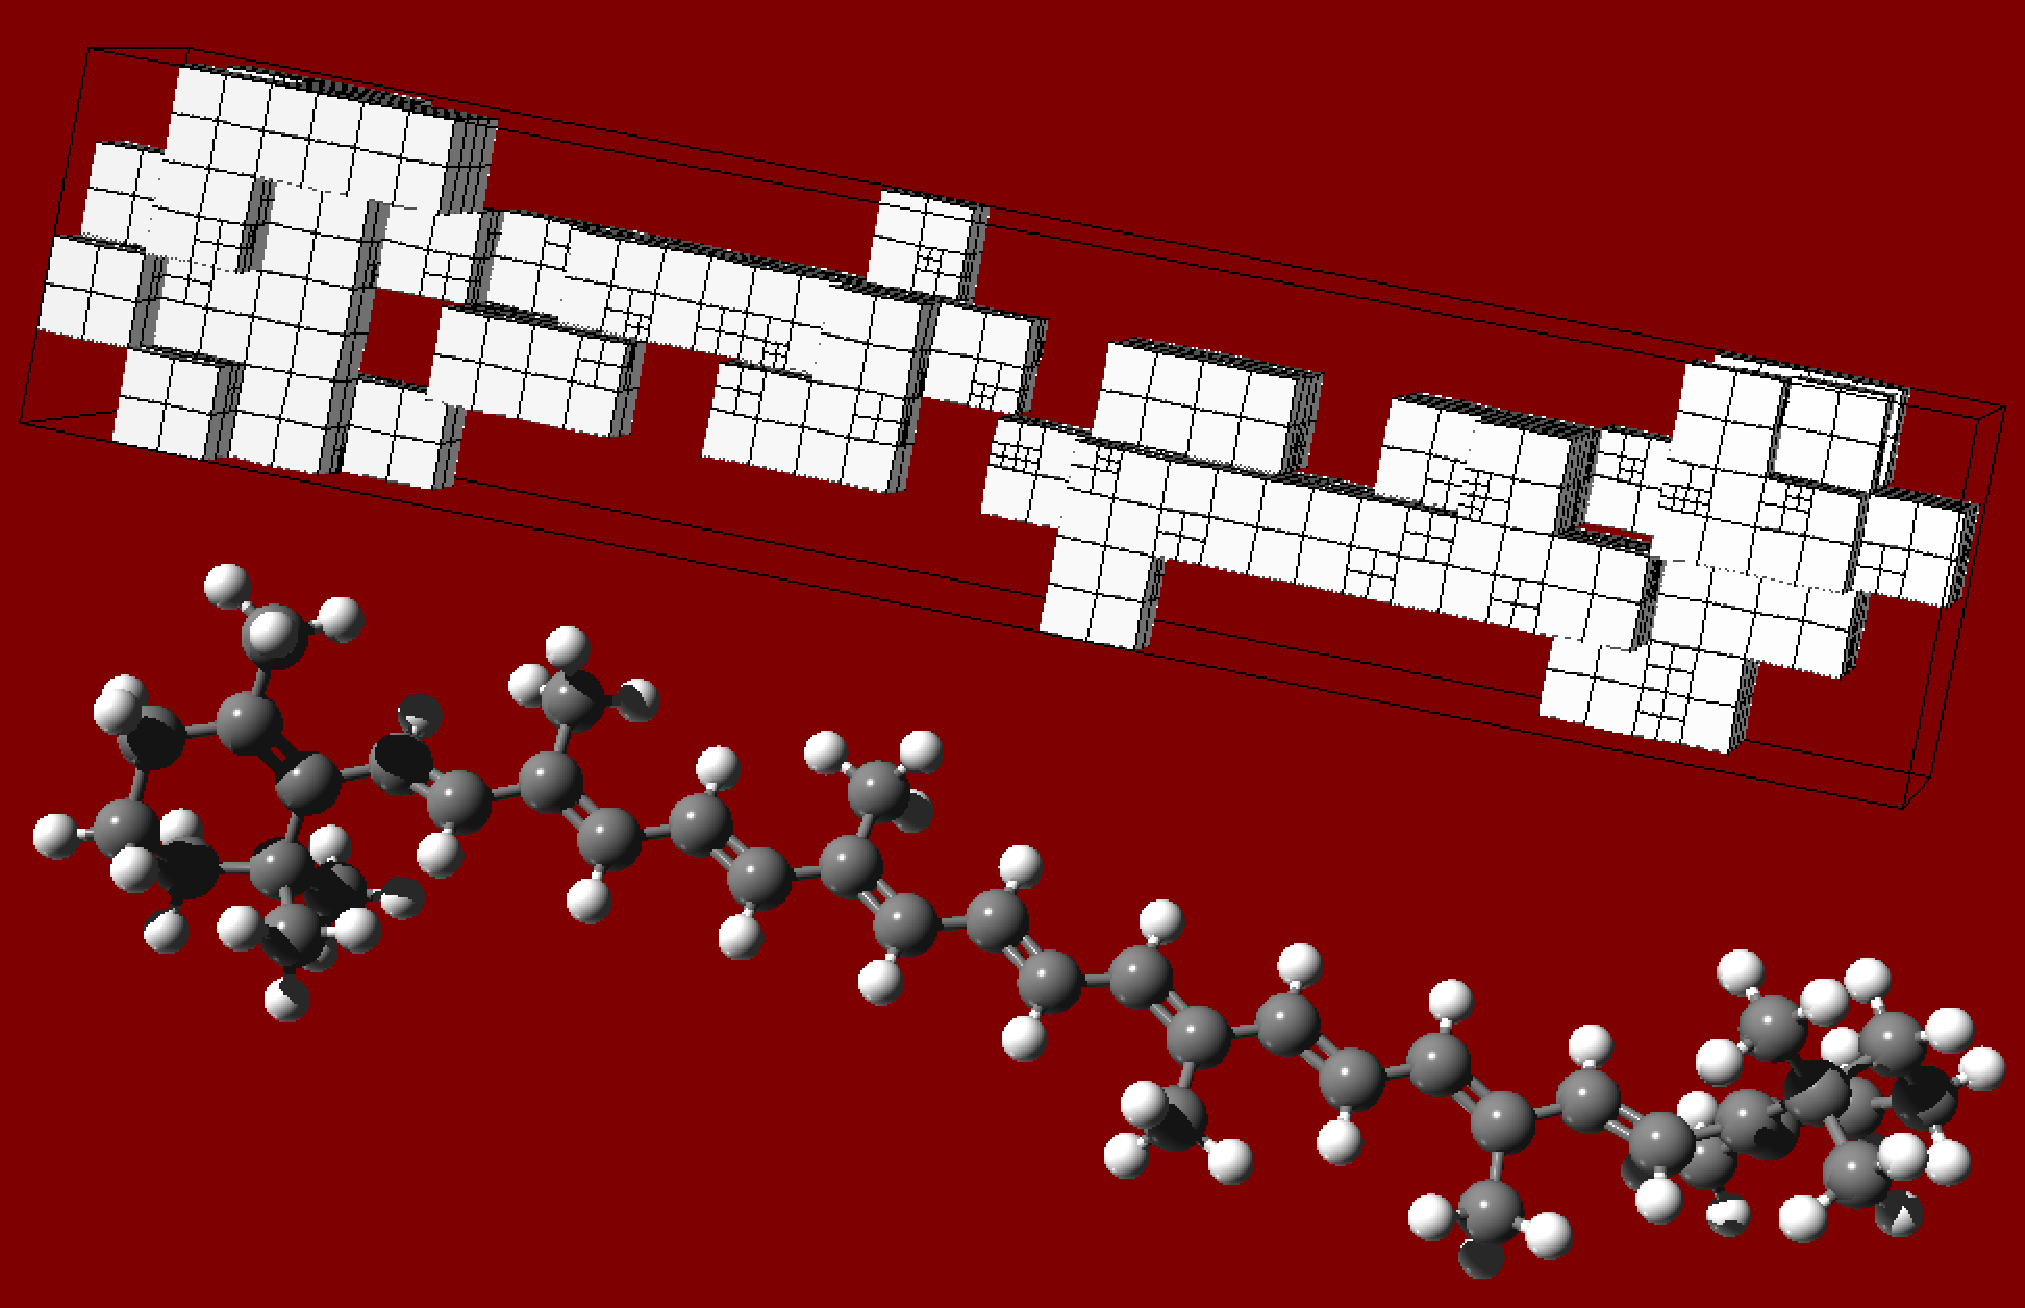
\includegraphics[angle=0, scale=0.2]{figures/caroteneGrid.pdf}
\end{frame}

\begin{frame}
    \frametitle{Integral formulation SCF}
    \begin{columns}
    \begin{column}{.5\textwidth}
    \centering
    \textbf{Effective potential}
    \begin{equation}
	\nonumber
	v_{eff}(\boldsymbol{r}) = v_\theta(\boldsymbol{r}) + v_{nuc}(\boldsymbol{r}) + 
	v_{el}(\boldsymbol{r}) + v_{xc}(\boldsymbol{r})
    \end{equation}
    \end{column}
    \begin{column}{.5\textwidth}
    \centering
    \textbf{Single orbital}
    \begin{equation}
	\nonumber
	\phi(\boldsymbol{r}) = \sqrt{\rho(\boldsymbol{r})}
    \end{equation}
    \end{column}
    \end{columns}
    \ \\
    \ \\
    \centering
    \textbf{OF-DFT Euler equation}
    \begin{equation}
	\nonumber
	\left[-\frac{1}{2}\nabla^2 + v_{eff}(\boldsymbol{r})\right]
	\phi(\boldsymbol{r}) =\ \mu \phi(\boldsymbol{r})
    \end{equation}
    \ \\
    \ \\
    \ \\
    \begin{itemize}
	\item	Invert the level-shifted laplacian $\left(-\nabla^2+k^2\right)$ using the bound-state Helmholtz Green's function
	\item	Integral equation solved iteratively to self-consistency
	\item	Standard iterative subspace acceleration techniques (KAIN or DIIS) can be applied
	\item	Fast and robust convergence for orbital-based SCF methods (KS-DFT and HF)
    \end{itemize}
    \ \\
    \ \\
    \ \\
    \begin{columns}
    \begin{column}{.5\textwidth}
    \centering
    \textbf{Rewritten in integral form}
    \begin{equation}
	\nonumber
	\phi(\boldsymbol{r}) =\ -2\int H^{\mu}(\boldsymbol{r}-\boldsymbol{r}')\
	    \Big[v_{eff}(\boldsymbol{r}') \phi(\boldsymbol{r}')\Big] d\boldsymbol{r}'
    \end{equation}
    \end{column}
    \begin{column}{.5\textwidth}
    \centering
    \textbf{Bound-state Helmholtz kernel}
    \begin{equation}
	\nonumber
	H^\mu(\boldsymbol{r}-\boldsymbol{r}') = \frac{e^{-\sqrt{-2\mu}|\boldsymbol{r}-\boldsymbol{r}'|}}{4\pi|\boldsymbol{r}-\boldsymbol{r}'|}
    \end{equation}
    \end{column}
    \end{columns}
    \ \\
    \ \\
    \textbf{Iterative solution}
    \begin{equation}
	\nonumber
	\phi^{n+1} =\ -2\hat{H}\left[v_{eff}^n\phi^n\right]
    \end{equation}
\end{frame}

\begin{frame}
    \frametitle{Results}
    \centering
    \textbf{Effective potential}
    \begin{equation}
	\nonumber
	v_{eff}(\boldsymbol{r}) = v_\theta(\boldsymbol{r}) + v_{nuc}(\boldsymbol{r}) + 
	v_{el}(\boldsymbol{r}) + v_{xc}(\boldsymbol{r})
    \end{equation}
    \ \\
    \ \\
    \begin{columns}
    \begin{column}{.5\textwidth}
    \centering
    \textbf{Thomas-Fermi kinetic potential}
    \begin{equation}
        \nonumber
	v_\theta(\boldsymbol{r})= -\frac{1}{2}\left(3\pi^2\right)^{2/3} \rho^{2/3}(\boldsymbol{r})
    \end{equation}
    \end{column}
    \begin{column}{.5\textwidth}
    \centering
    \textbf{Slater-Dirac exchange potential}
    \begin{equation}
        \nonumber
	v_{xc}(\boldsymbol{r}) = -\left(\frac{3}{\pi}\right)^{1/3} \rho^{1/3}(\boldsymbol{r})
    \end{equation}
    \end{column}
    \end{columns}
    \ \\
    \ \\
    \begin{itemize}
	\item	Two methods: Dirac-von Weizs\"{a}cker (DvW) and Thomas-Fermi-Dirac-von Weizs\"{a}cker (TFDvW)
	\item	Convergence \textbf{very problematic} for many-electron systems when TF is included
	\item	Had to introduce TF gradually to avoid divergence (add 2\% TF and converge to $10^{-2}$)
	\item	The Borgoo-Tozer functional did not converge for any system
    \end{itemize}
    \ \\
    \centering
    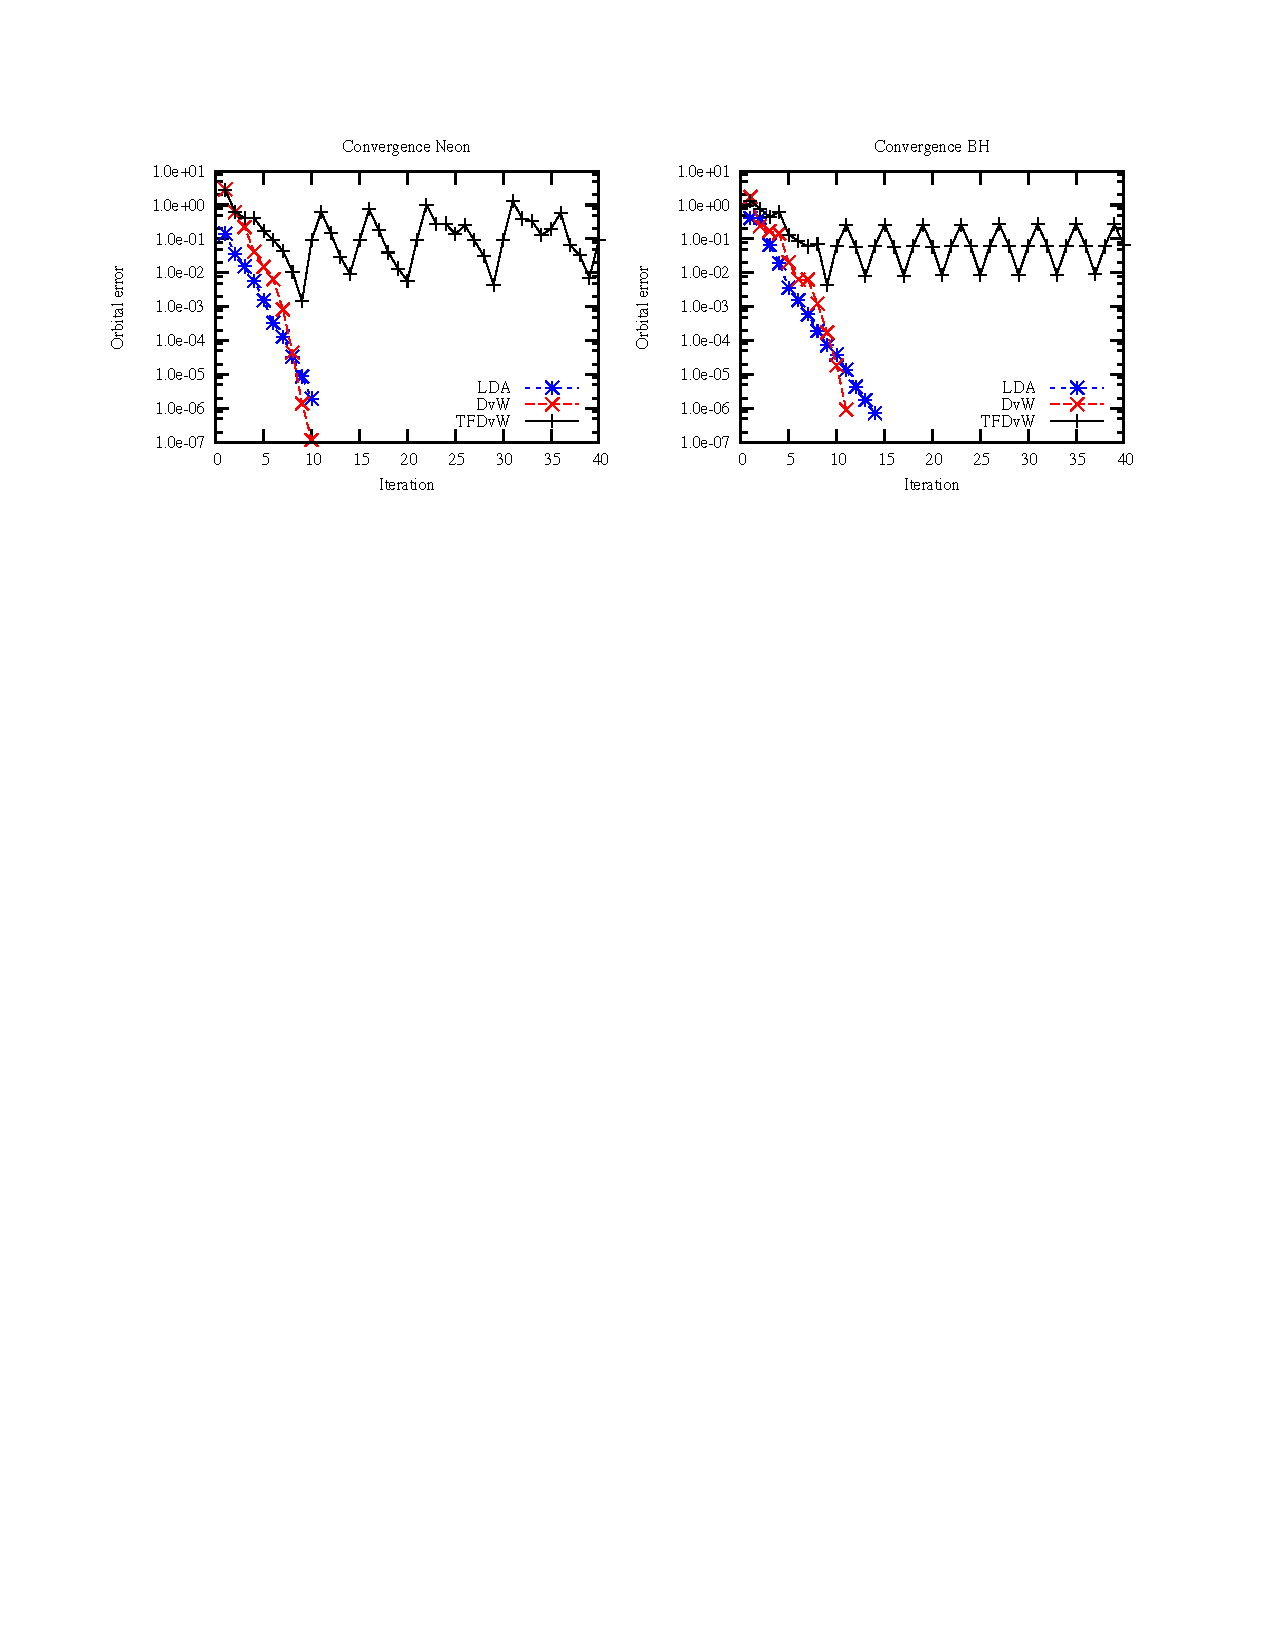
\includegraphics[scale=0.6, viewport = 50 560 550 730]{figures/convergence.pdf}\\
\end{frame}

\begin{frame}
    \frametitle{Results}
\begin{table}
\footnotesize
\begin{center}
\begin{tabular}{ll|ll|llll}
\hline
\hline
	&		    &               &               &               &               &               &		    \\
	&		    &\multicolumn{2}{|c|}{Chemical potential}&\multicolumn{4}{|c}{Total energy (Hartree)}\\
	&		    &               &               &               &               &               &		    \\
	&		    &
\multicolumn{1}{|c}{DvW}&
\multicolumn{1}{c|}{TFDvW}&
\multicolumn{1}{c}{DvW}&
\multicolumn{1}{c}{TFDvW}&
\multicolumn{1}{c}{LDA}&
\multicolumn{1}{c}{RHF}\\
	&		    &               &               &               &               &               &		    \\
\hline                                                      
	&		    &               &               &               &               &               &		    \\
H	& MRChem	    &  -0.194320    &  -0.071640    &   -0.406534   &  -0.261826    &   -0.406534   &   -0.500000   \\
	& Chan$^\dag$	    &		    &  -0.071	    &		    &  -0.2618      &		    &   -0.5000     \\
        & Karasiev$^\ddag$  &  -0.1943      &  -0.0715      &   -0.406534   &  -0.261827    &   -0.4065     &		    \\
	&		    &               &               &               &               &               &		    \\
	&		    &               &               &               &               &               &		    \\
Ne	& MRChem	    &  -7.060692    &  -0.180760    & -274.680827   & -85.734479    & -127.490748   & -128.547101   \\
	& Chan$^\dag$	    &		    &  -0.181       &		    & -85.7343      &		    & -128.5471     \\
	& Karasiev$^\ddag$  &  -7.0607	    &  -0.1807      & -274.68080    & -85.734451    & -127.4907	    &		    \\
	&		    &               &               &               &               &               &		    \\
	&		    &               &               &               &               &               &		    \\
H$_2$	& MRChem	    &  -0.331330    &  -0.100168    &   -1.043736   &  -0.43072     &   -1.043736   &   -1.133619   \\
BH	& MRChem	    &  -1.170066    &  -0.146852    &  -38.589138   & -15.301851    &  -24.629804   &  -25.131640   \\
	&		    &               &               &               &               &               &		    \\
\hline                                                                                  
\hline                                                                                  
\end{tabular}
\end{center}
\end{table}
\ \\
\ \\
\ \\
\ \\
\centering
$^\dag$\tiny{Chan, Cohen, Handy, \it{J. Chem. Phys.} \textbf{114}, 631 (2001)}\\
$^\ddag$\tiny{Karasiev, Trickey, \it{Comp. Phys. Comm.} \textbf{121(5)}, 2030 (2012)}
\end{frame}

\begin{frame}
    \frametitle{Results}
    \centering
    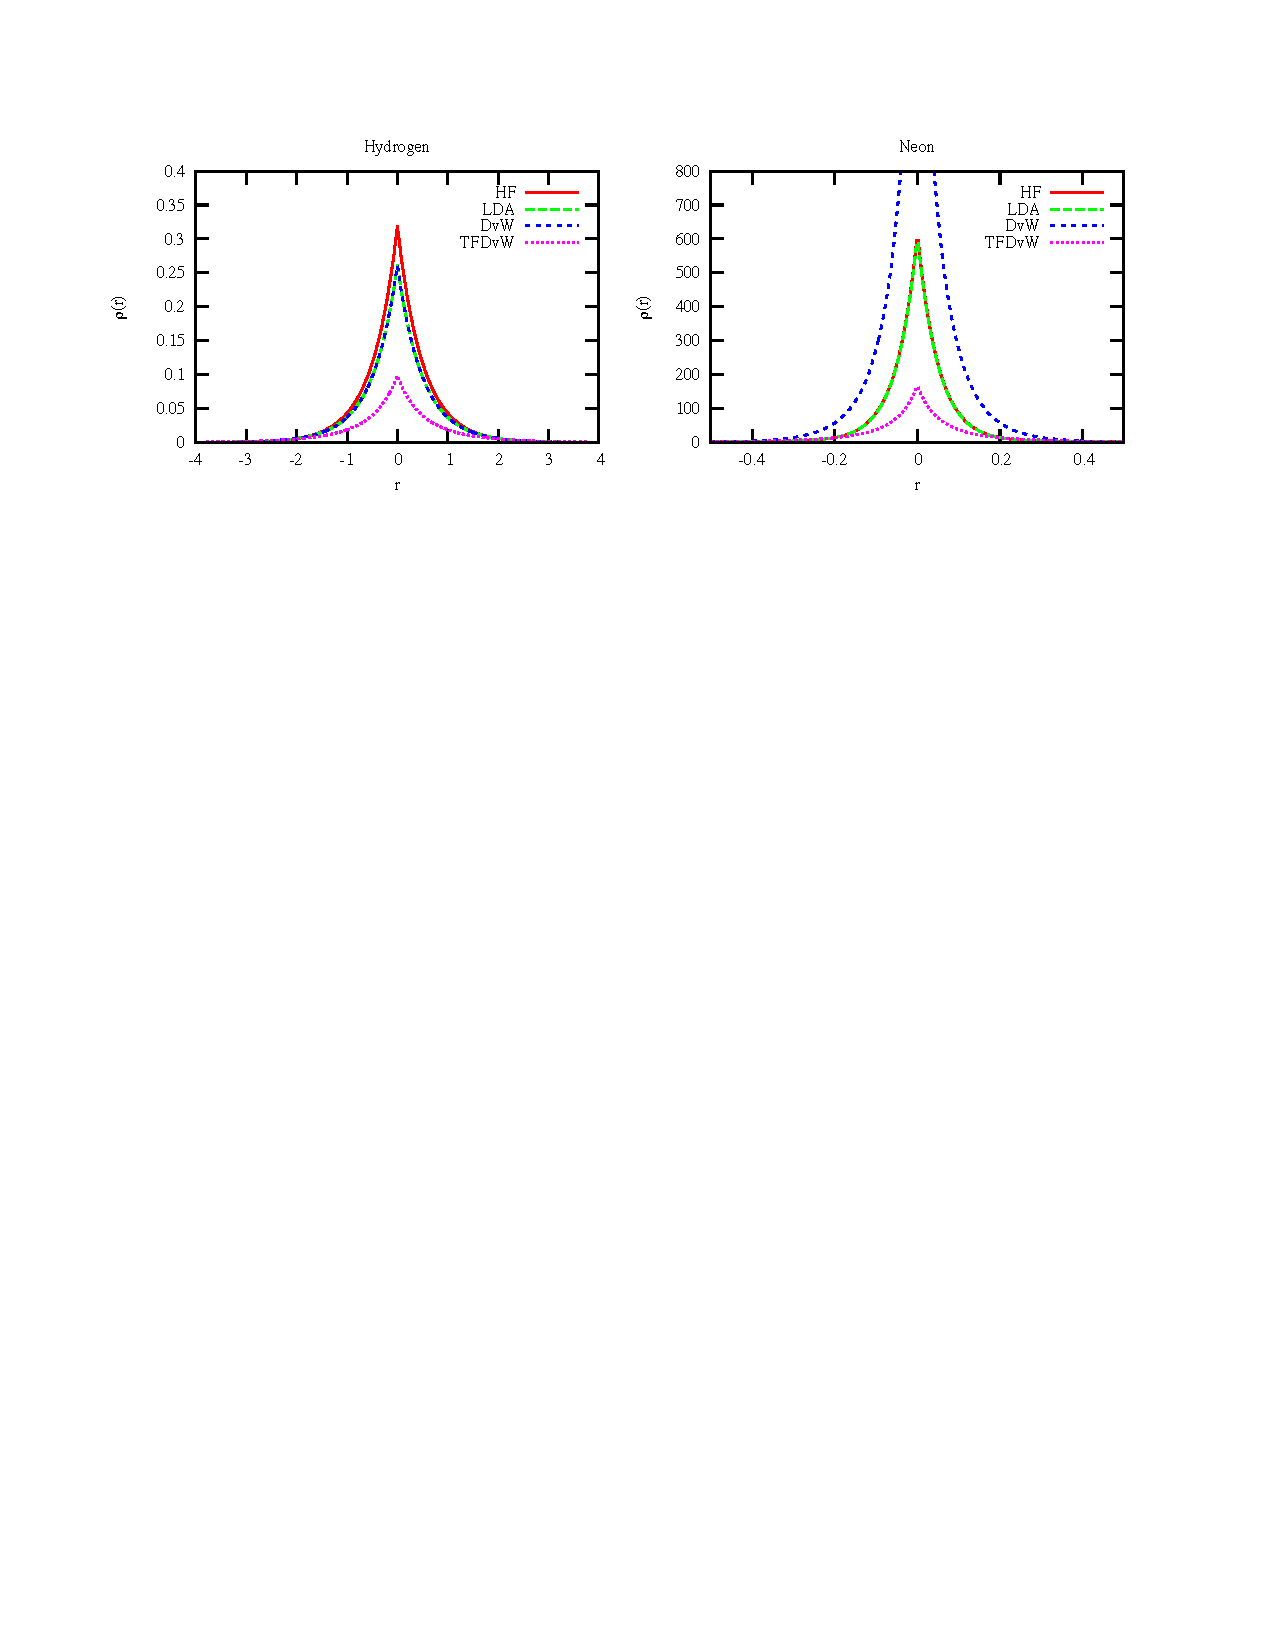
\includegraphics[scale=0.6, viewport = 50 560 550 755]{figures/of_atoms.pdf}\\
    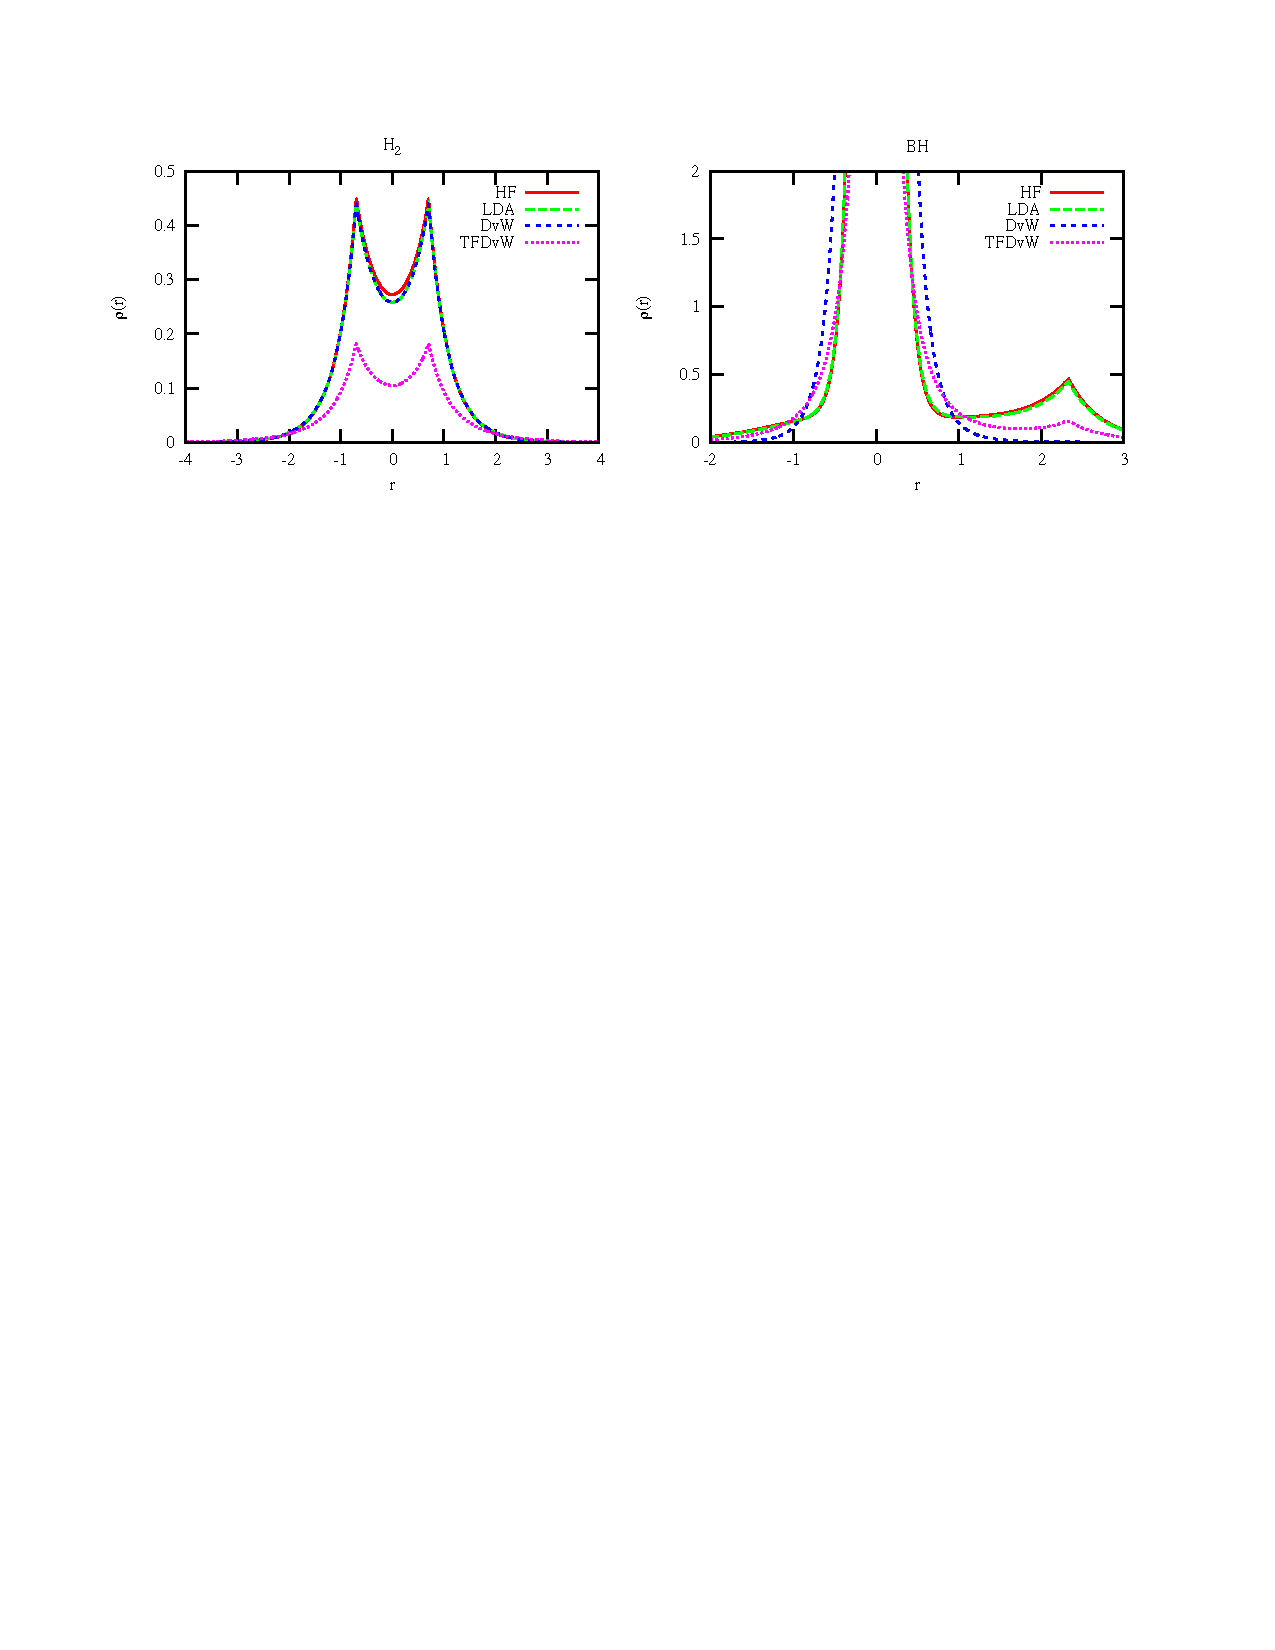
\includegraphics[scale=0.6, viewport = 50 560 550 755]{figures/of_molecules.pdf}
    \ \\
    \ \\
    \ \\
\end{frame}

\begin{frame}
    \frametitle{Conclusions and outlook}
    \begin{itemize}
	\item	Formulation as one-orbital Kohn-Sham problem is \textbf{not appropriate}
	\item	Convergence is very sensitive to the repulsive Thomas-Fermi potential
	\item	Very high accuracy was easily attained once the full Thomas-Fermi was included
	\item	Borgoo-Tozer functional did not converge for any system
    \end{itemize}
    \ \\
    \ \\
    \ \\
    \ \\
    \ \\
    \begin{itemize}
	\item	Multiwavelets can still be the ideal framework for developing new functionals
	\item	Remove one source of error (basis set)
	\item	Involves only a few global functions that are easily parallelized 
	\item	Requires a different and more robust optimization algorithm (2nd order Newton-Raphson?)
    \end{itemize}
\end{frame}

\end{document}
